% 图 1：状态空间系统框图（开环）
\documentclass[border=6pt]{standalone}
% 四张示意图共用的字体、颜色与 TikZ 设置
\usepackage{fontspec}
\usepackage{xeCJK}
\setmainfont{TeX Gyre Pagella}
\setCJKmainfont{Noto Serif CJK SC}[AutoFakeSlant=0.15]
\usepackage{unicode-math}
\setmathfont{TeX Gyre Pagella Math}
\usepackage{amsmath}
\usepackage{tikz}
\usetikzlibrary{arrows.meta, positioning, calc, decorations.markings, backgrounds, fit, shapes.geometric}

\definecolor{navy}{HTML}{1E3A8A}
\definecolor{teal}{HTML}{0F766E}
\definecolor{amber}{HTML}{B45309}
\definecolor{softblue}{HTML}{EFF6FF}
\definecolor{softteal}{HTML}{F0FDFA}
\definecolor{softamber}{HTML}{FFFBEB}
\definecolor{border}{HTML}{CBD5E1}
\definecolor{graytext}{HTML}{5B6673}
\definecolor{redalert}{HTML}{991B1B}

\tikzset{
  >=Latex,
  every node/.style={font=\small},
  block/.style={draw=navy, thick, rounded corners=3pt, fill=softblue, align=center},
  bus/.style={thick, graytext},
}

\begin{document}
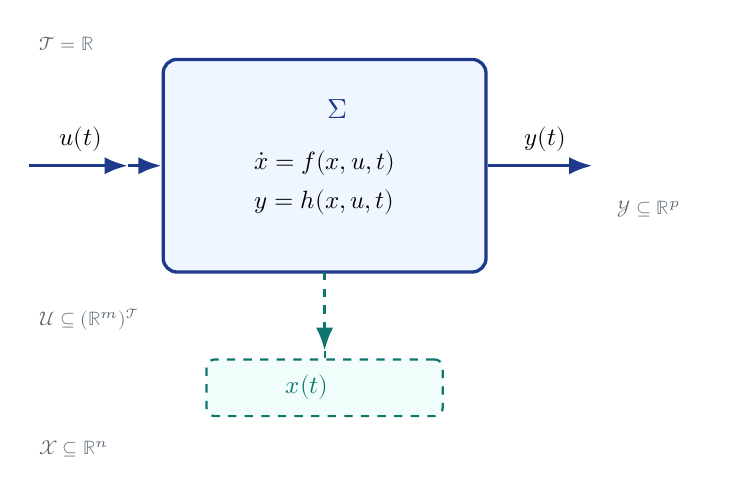
\begin{tikzpicture}[x=1cm,y=1cm]
  % 输入
  \draw[->, very thick, navy] (-2.6,0) -- (-1.35,0);
  \node[above] at (-1.95,0.05) {$u(t)$};
  \node[below, text=graytext] at (-1.95,-0.08) {输入};

  % 系统方框
  \node[draw=navy, very thick, rounded corners=5pt, fill=softblue,
        minimum width=4.1cm, minimum height=2.7cm] (sys) at (1.15,0) {};
  \node[text=navy, font=\bfseries] at (1.15,0.72) {系统 $\Sigma$};
  \node[align=center] at (1.15,-0.22) {$\dot x=f(x,u,t)$\\[3pt]$y=h(x,u,t)$};

  \draw[->, very thick, navy] (-1.35,0) -- (sys.west);
  \draw[->, very thick, navy] (sys.east) -- (4.55,0);
  \node[above] at (3.95,0.05) {$y(t)$};
  \node[below, text=graytext] at (3.95,-0.08) {输出};

  % 状态引出
  \draw[->, dashed, very thick, teal] (1.15,-1.35) -- (1.15,-2.35);
  \node[draw=teal, dashed, thick, rounded corners=3pt, fill=softteal,
        text=teal, minimum width=3.0cm, minimum height=0.72cm] (state) at (1.15,-2.82)
        {$x(t)$：内部状态};
  \draw[dashed, thick, teal] (1.15,-2.35) -- (state.north);

  % 空间标注（放在空白处，避免与方框和状态引线重叠）
  \node[text=graytext, anchor=west, font=\scriptsize] at (-2.6,1.55)
        {$\mathcal T=\mathbb R$（连续时间）};
  \node[text=graytext, anchor=west, font=\scriptsize] at (-2.6,-1.95)
        {$\mathcal U\subseteq(\mathbb R^m)^{\mathcal T}$};
  \node[text=graytext, anchor=west, font=\scriptsize] at (-2.6,-3.60)
        {$\mathcal X\subseteq\mathbb R^n$（状态空间）};
  \node[text=graytext, anchor=west, font=\scriptsize] at (4.75,-0.55)
        {$\mathcal Y\subseteq\mathbb R^p$（输出空间）};
\end{tikzpicture}
\end{document}
